\documentclass[12pt, a4paper]{article}
\usepackage[utf8]{inputenc}
\usepackage{polski}
\usepackage{hyperref}
\usepackage{float}
\usepackage{algorithm}
\usepackage{algpseudocode}
\usepackage{geometry}
\usepackage[table]{xcolor}
\usepackage{graphicx}
\usepackage{subfigure}
\title{\textbf{Zastosowanie algorytmu ewolucyjnego do rozwiązywania problemu komiwojażera}}
\author{Anna Stępień \\ Adam Stelmaszczyk}
\date{\today}
\setlength{\parindent}{0in}
\makeatletter\renewcommand{\ALG@name}{}

\begin{document}
\maketitle

\section{Zadanie}
Celem zadania jest zaprojektowanie algorytmu ewolucyjnego, który zostanie wykorzystany do rozwiązania problemu komiwojażera.
Przedstawiona została reprezentacja rozwiązania, metoda sukcesji oraz operatory mutacji i krzyżowania. 
Z punktu widzenia przydatności projektowanego algorytmu, istotne jest przetestowanie go dla różnych parametrów, w szczególności dla:
\begin{itemize}
	\item różnych wartości prawdopodobieństwa mutacji $p_m$ i krzyżowania $p_c$,
	\item grafów o różnej liczbie wierzchołków $d$.
\end{itemize}

\section{Założenia}
Aplikacja będzie pracować w trybie konsolowym. Na standardowe wejście podawane będą pliki tekstowe zawierające opis grafów.
Program będzie wypisywał odpowiedź na standardowe wyjście.

\subsection{Reprezentacja rozwiązań}

Wierzchołki grafu numerujemy od 0 do $d - 1$. Zakładamy, że $d \in \mathcal{N}$ oraz $d \geq 3$. 
Rozwiązania reprezentujemy jako wektory złożone z $d$ unikalnych liczb. 
Np. $[0,1,2]$ oznacza rozwiązanie złożone z 3 krawędzi: $(0,1), (1,2), (2,0)$. 
W ogólnym przypadku, dla grafu pełnego o $d$ wierzchołkach, liczba unikalnych rozwiązań wynosi $\frac{(d-1)!}{2}$. 
Minimalizowana wartość funkcji celu $f$ to suma wag krawędzi w cyklu dla danego rozwiązania.

\section{Projekt rozwiązania}

\subsection{Schemat algorytmu ewolucyjnego}

\begin{algorithm}[!htb]
\label{ea}
\begin{algorithmic}[1]
\Function{algorytm\_ewolucyjny}{}
  \State $P(0) \gets \{x_1, x_2, \ldots, x_n\}$
  \State $t \gets 0$
  \While{$! stop$}
    \For{$i = 0$ \bf{to} $i = n - 1$}
      \State $a \gets$ selekcja$(P(t))$
      \If{$\mathcal{U}(0, 1) < p_c$}
	\State $b \gets$ selekcja$(P(t))$
	\State $O(t,i) \gets$ mutacja$($krzy{\.z}owanie$(a, b))$
      \Else
	\State $O(t,i) \gets$ mutacja$(a)$
      \EndIf
    \EndFor
    \State $P(t+1) \gets$ sukcesja$(P(t),O(t))$
    \State $t \gets t+1$
  \EndWhile
\EndFunction
\end{algorithmic}
\end{algorithm}

\subsubsection{Mutacja}

Operator mutacji otrzymuje na wejściu prawdopodobieństwo mutacji $p_m$ oraz rozwiązanie długości $d$.
Zwraca rozwiązanie długości $d$, nazywane mutantem.

\begin{enumerate}
 \item Utwórz początkowego mutanta kopiując rozwiązanie wejściowe.
 \item Liczba powtórzeń $R = \lceil d \cdot  p_m \rceil$. Powtórz $R$ razy następujące kroki:
 \item Wylosuj dwa różne indeksy $i, j$ od 0 do $d-1$ zgodnie z rozkładem jednostajnym.
 \item Zamień liczbę na pozycji $i$-tej z liczbą na pozycji $j$-tej w mutancie.
\end{enumerate}

\subsubsection{Krzyżowanie}

Operator krzyżowania na wejściu otrzymuje dwa rozwiązania rodzicielskie długości $d$ i zwraca jedno rozwiązanie potomne długości $d$. 
Jako operator krzyżowania zostanie wykorzystany 
Order1\footnote{\url{http://www.rubicite.com/Tutorials/GeneticAlgorithms/CrossoverOperators/Order1CrossoverOperator.aspx}}:
\begin{enumerate}
 \item Wylosuj dwa indeksy $i, j$ od 0 do $d-1$ zgodnie z rozkładem jednostajnym.
 \item Utwórz jedno puste rozwiązanie potomne długości $d$.
 \item Skopiuj miasta od $i$ do $j$ z pierwszego rodzica do potomka.
 \item Począwszy od lewej strony, wypełnij kolejno puste miejsca potomka tymi miastami drugiego z rodziców, 
których nie ma w skopiowanej sekwencji.
\end{enumerate}

Przykład: \\

Wejściowe rozwiązania rodzicielskie: \\

Rodzic 1
\begin{tabular}{ | c | c | c | c | c | c | c | c |}
  \hline
  2 & 6 &  \cellcolor{green!25}7 & \cellcolor{green!25}1 & \cellcolor{green!25}5 & \cellcolor{green!25}4 & 8 & 3 \\ \hline
\end{tabular}\\
Rodzic 2
\begin{tabular}{ | c | c | c | c | c | c | c | c |}
  \hline
  7 & 5 & 6 & 3 & 8 & 2 & 1 & 4 \\ \hline
\end{tabular}

\begin{enumerate}
 \item Wylosowano $i = 2$, $j = 5$.

 \item Początkowo pusty potomek:
\begin{tabular}{ | c | c | c | c | c | c | c | c |}
 \hline
   &  &  &  &  &  &  &  \\ \hline
\end{tabular}

 \item Skopiowanie sekwencji od $i$ do $j$:
\begin{tabular}{ | c | c | c | c | c | c | c | c |}
 \hline
   &  &  \cellcolor{green!25}7 & \cellcolor{green!25}1 & \cellcolor{green!25}5 & \cellcolor{green!25}4 &  &  \\ \hline
\end{tabular}

 \item Iterujemy przez miasta drugiego rodzica, zaczynamy od 7. 7 już jest w potomku, więc przesuwamy się w prawo.
5 również jest już w potomku, przesuwamy się w prawo. 6 nie ma w potomku, także ją wstawiamy w pierwszym wolnym miejscu
i przesuwamy się w prawo. 3 wstawiamy, 8 i 2 też, 1 i 4 nie. Wyjściowy potomek:

\begin{tabular}{ | c | c | c | c | c | c | c | c |}
 \hline
  6 & 3 &  \cellcolor{green!25}7 & \cellcolor{green!25}1 & \cellcolor{green!25}5 & \cellcolor{green!25}4 & 8 & 2 \\ \hline
\end{tabular}\\

\end{enumerate}

\subsubsection{Selekcja}

Operator selekcji otrzymuje na wejściu populację o rozmiarze $n$. Zwraca jedno losowe rozwiązanie z populacji wejściowej
zgodnie z rozkładem jednostajnym.

\subsubsection{Sukcesja}

Metoda sukcesji na wejściu otrzymuje dwie populacje o rozmiarze $n$: aktualną $P$ oraz populację mutantów $O$.
Wyjściem jest jedna populacja o rozmiarze $n$.

\begin{algorithm}[!htb]
\begin{algorithmic}[1]
\Function{sukcesja}{}
  \For{$i = 0$ \bf{to} $i = n - 1$}
    \If{$f(O(t, i)) < f(P(t, i)) $}
      \State $P(t+1, i) \gets O(t, i)$
    \Else
      \State $P(t+1, i) \gets P(t, i)$
    \EndIf
  \EndFor
\EndFunction
\end{algorithmic}
\end{algorithm}

\subsection{Struktury danych}
	\paragraph{Rozwiązanie}
		Rozwiązanie jest reprezentowane jako tablica $d$ liczb całkowitych, której elementy są numerami miast.
	\paragraph{Populacja}
		Populacja jest reprezentowana jako tablica rozwiązań. Rozmiar populacji jest stały i równy $n = 10d$.

\subsection{Założenia programu}
\begin{description}
	\item[Wejście] \hfill \\
Wejściem dla algorytmu jest graf nieskierowany dany macierzą o~$n$~wierszach i~$n$~kolumnach:

\bigskip
$ 
\begin{array}{llll}
n \\
q_{0,0} & q_{1,0} & \ldots & q_{n-1,0} \\
q_{0,1} & q_{1,1} & \ldots & q_{n-1,1} \\
\vdots  & \vdots  & \ddots & \vdots  \\
q_{0,n-1} & q_{1,n-1} & \ldots & q_{n-1,n-1} 
\end{array}
, q_{i,j} \in \{0,1\}, 0 \leq i,j < n
$
\bigskip

$q_{i,j}$ oznacza wagę krawędzi pomiędzy wierzchołkami $i$ i $j$.
\par\vspace{\baselineskip}
Macierz jest dana w pliku tekstowym, w którym kolejne $q_{i,j}$ w wierszu $j$ są oddzielone co najmniej jednym znakiem białym. Przez znak biały rozumiemy
spację lub tabulator. Pierwszy wiersz pliku zawiera wymiar macierzy.
>>>>>>> Stashed changes

Poniżej przedstawiono przykładowy, poprawny plik wejściowy:

\bigskip
$ 
\begin{array}{llll}
4 \\
0.0 & 1.0 & 3.6 & 2.0 \\
1.0 & 0.0 & 2.8 & 2.2 \\
3.6 & 2.8 & 0.0 & 3.0 \\
2.0 & 2.2 & 3.0 & 0.0
\end{array}
$
	\item[Wyjście] \hfill \\
	Wyjściem algorytmu jest plik tekstowy zawierający koszt najtańszego cyklu znalezionego przez algorytm.
	\item[Kryteria stopu] \hfill \\
	Warunkiem zatrzymania algorytmu jest wywołanie $10^5d$ razy funkcji oceny, gdzie $d$ to rozmiar problemu (liczba miast).
	\item[Parametry] \hfill \\
	Na wejście programu możliwe jest podanie dwóch parametrów określających odpowiednio:
		\begin{itemize}
			\item prawdopodobieństwo mutacji $p_m$ (domyślna wartość 0,9)
			\item prawdopodobieństwo krzyżowania $p_c$ (domyślna wartość 0,1)
		\end{itemize}
		W przypadku, gdy parametry te nie zostaną sprecyzowane, stosowane są wartości domyślne.
	\item[Złożoność obliczeniowa] \hfill \\
	Złożoność obliczeniowa operatorów genetycznych: mutacji oraz krzyżowania jest równa $O(d)$, 
gdzie $d$ to rozmiar rozwiązania (liczba miast). Złożoność obliczeniowa selekcji wynosi $O(1)$. Złożoność obliczeniowa
sukcesji jest liniowa względem liczby rozwiązań w populacji $n$, czyli $O(n)$. 
	\item[Sytuacje awaryjne] \hfill \\
Problemami, które mogą wystąpić podczas działania aplikacji są:
	\begin{itemize}
        \item błędny format danych wejściowych,
        \item błędny format parametrów aplikacji.
	\end{itemize}

W przypadku, gdy algorytm otrzyma na wejściu błędne dane np. liczba wierszy macierzy będzie niezgodna z zadeklarowaną na początku pliku z danymi lub , użytkownik zostanie poinformowany o zaistniałej sytuacji, a dalsze działanie programu zostanie przerwane.

\end{description}

\section{Projekt testów}
W ramach testów działanie algorytmu ewolucyjnego zostanie zweryfikowane dla szeregu problemów o~różniej wielkości. Szczególnie istotne jest zbadanie skuteczności algorytmu w~zależności od doboru wartości:
\begin{itemize}
	\item prawdopodobieństwa mutacji $p_m$,
	\item prawdopodobieństwa krzyżowania $p_c$.
\end{itemize}

Podczas testowania będziemy analizować następujące kombinacje wartości wartości prawdopodobieństwa mutacji $(p_m)$ i prawdopodobieństwa krzyżowania $(p_c)$.

\bigskip

Dla ustalonej wartości $p_c = 0,9$ - zbadanie wpływu zmian $p_m$:
\begin{center}
\begin{tabular}{|l|l|l|l|}
\hline
\multicolumn{4}{|c|}{$(p_c; p_m)$} \\
\hline
(0,9; 0,1) & (0,9; 0,5) & (0,9; 0,9) & (0,9; 1)\\
\hline
\end{tabular}
\end{center}

\bigskip

Dla ustalonej wartości $p_m = 0,1$ - zbadanie wpływu zmian $p_c$:
\begin{center}
\begin{tabular}{|l|l|l|l|}
\hline
\multicolumn{4}{|c|}{$(p_c; p_m)$} \\
\hline
(0,1; 0,1) & (0,5; 0,1) & (0,9; 0,1) & (1; 0,1)\\
\hline
\end{tabular}
\end{center}

\bigskip

Dla wyłączonej mutacji $p_m = 0$ - zbadanie wpływu zmian $p_c$
\begin{center}
\begin{tabular}{|l|l|l|l|}
\hline
\multicolumn{4}{|c|}{$(p_c$, $p_m)$} \\
\hline
(0,1; 0) & (0,5; 0) & (0,9; 0) & (1; 0)\\
\hline
\end{tabular}
\end{center}

\bigskip

Dla wyłączonego krzyżowania $p_c = 0$ - zbadanie wpływu zmian $p_m$
\begin{center}
\begin{tabular}{|l|l|l|l|}
\hline
\multicolumn{4}{|c|}{$(p_c$, $p_m)$} \\
\hline
(0; 0,1) & (0; 0,5) & (0; 0,9) & (0; 1)\\
\hline
\end{tabular}
\end{center}

\bigskip
Pojedynczy przypadek testowy polega na uruchomieniu algorytmu ewolucyjnego dla określonego problemu i zadanych wartości prawdopodobieństwa mutacji $p_m$ i prawdopodobieństwa krzyżowania $p_c$. Każdy przypadek testowy uruchomiony będzie niezależnie $RUNS = 15$ razy.

Poszczególne przypadki testowe będą uruchamiane dla ustalonej wartości ziarna generatora liczb pseudolosowych -- w ten sposób sekwencje liczb pseudolosowych dla każdej wersji algorytmu będą jednakowe, co umożliwi porównanie ich skuteczności.

Do testowania zaimplementowanego algorytmu ewolucyjnego wykorzystane zostaną zestawy danych, dla których z~góry znany jest koszt optymalnego cyklu. W~celu porównania skuteczności poszczególnych ustawień algorytmu, dla każdego z~przypadków testowych zostaną wykreślone dystrybuanty empiryczne -- miarą jakości algorytmu będzie różnica pomiędzy optymalnym kosztem cyklu a~kosztem obliczonym przez algorytm.

\section{Wyniki testów}
\subsection{Wpływ prawdopodobieństwa mutacji}
\begin{figure}[H]
\centering
\mbox{\subfigure[$p_c = 0,9$]{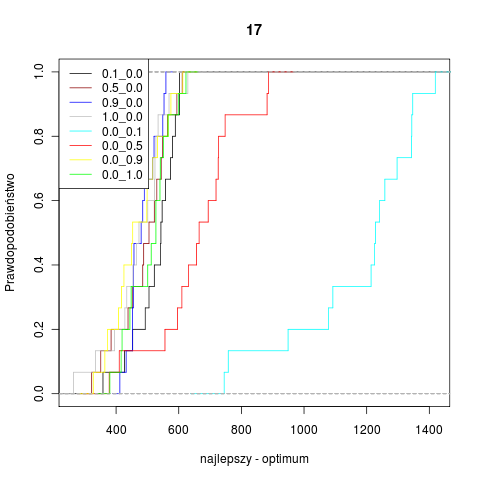
\includegraphics[width=.5\textwidth]{../tests/normal/17.png} }\quad
\subfigure[$p_c = 0$ - wyłączone krzyżowanie]{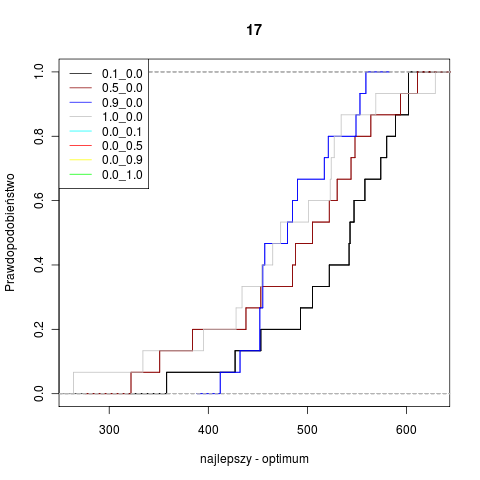
\includegraphics[width=.5\textwidth]{../tests/normal/17m.png} } 
}
\caption{Wpływ mutacji na działanie algorytmu - 17 miast}
\end{figure}

\begin{figure}[H]
\centering
\mbox{\subfigure[$p_c = 0,9$]{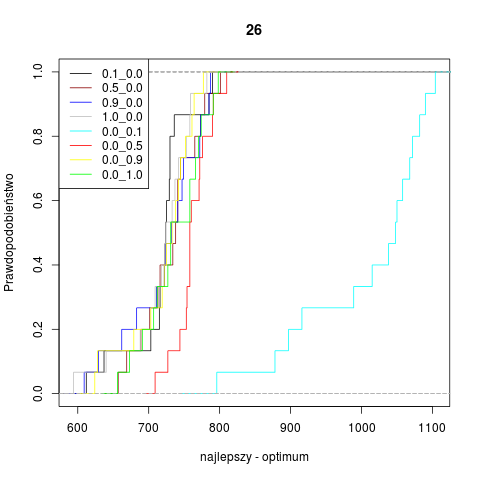
\includegraphics[width=.5\textwidth]{../tests/normal/26.png} }\quad
\subfigure[$p_c = 0$ - wyłączone krzyżowanie]{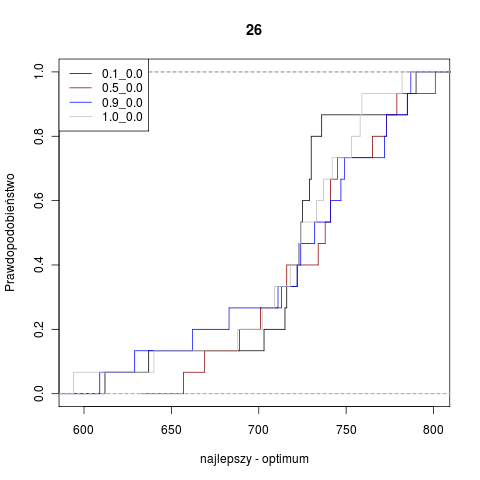
\includegraphics[width=.5\textwidth]{../tests/normal/26m.png} } 
}
\caption{Wpływ mutacji na działanie algorytmu - 26 miast}
\end{figure}

\begin{figure}[H]
\centering
\mbox{\subfigure[$p_c = 0,9$]{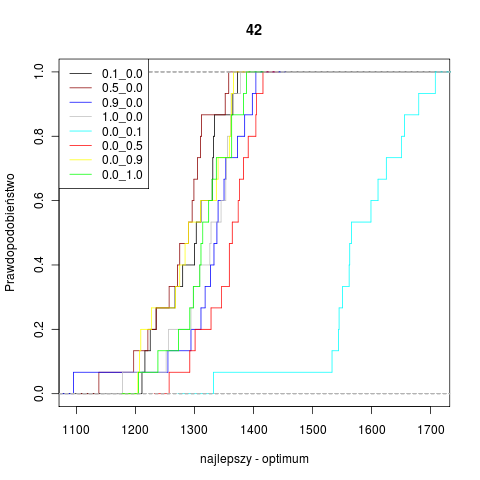
\includegraphics[width=.5\textwidth]{../tests/normal/42.png} }\quad
\subfigure[$p_c = 0$ - wyłączone krzyżowanie]{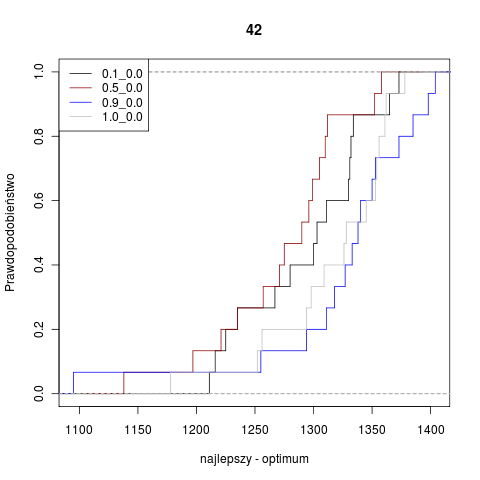
\includegraphics[width=.5\textwidth]{../tests/normal/42m.png} } 
}
\caption{Wpływ mutacji na działanie algorytmu - 42 miasta}
\end{figure}

\begin{figure}[H]
\centering
\mbox{\subfigure[$p_c = 0,9$]{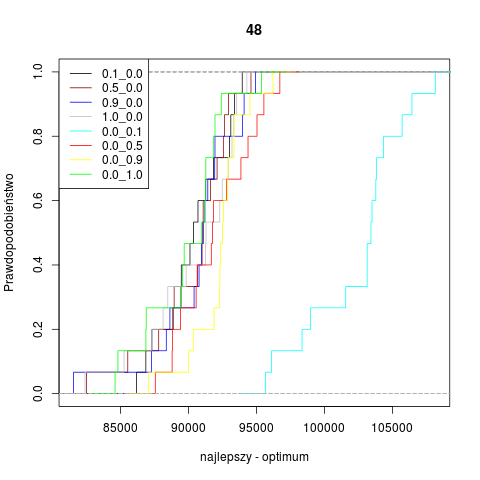
\includegraphics[width=.5\textwidth]{../tests/normal/48.png} }\quad
\subfigure[$p_c = 0$ - wyłączone krzyżowanie]{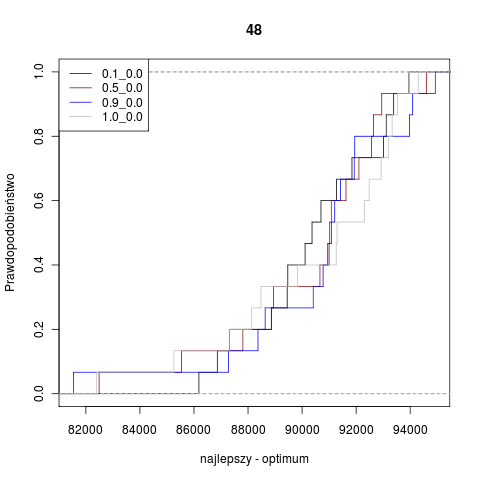
\includegraphics[width=.5\textwidth]{../tests/normal/48m.png} } 
}
\caption{Wpływ mutacji na działanie algorytmu - 48 miast}
\end{figure}

\subsection{Wpływ prawdopodobieństwa krzyżowania}
\begin{figure}[H]
\centering
\mbox{\subfigure[$p_m = 0,1$]{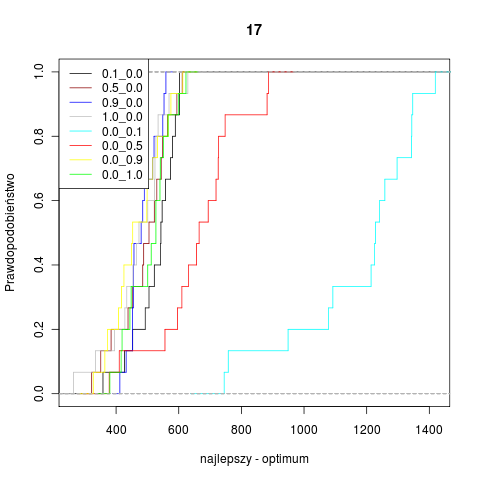
\includegraphics[width=.5\textwidth]{../tests/normal/17.png} }\quad
\subfigure[$p_m = 0$ - wyłączona mutacja]{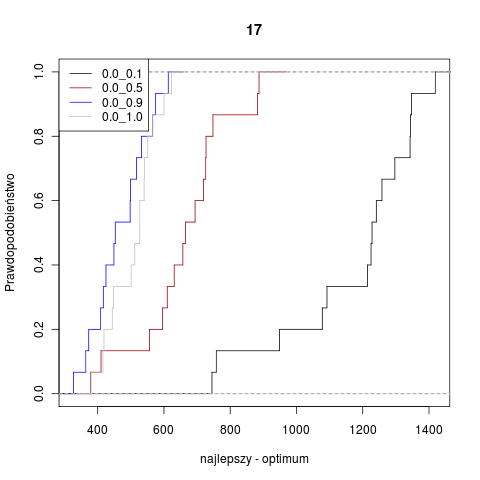
\includegraphics[width=.5\textwidth]{../tests/normal/17c.png} } 
}
\caption{Wpływ krzyżowania na działanie algorytmu - 17 miast}
\end{figure}

\begin{figure}[H]
\centering
\mbox{\subfigure[$p_m = 0,1$]{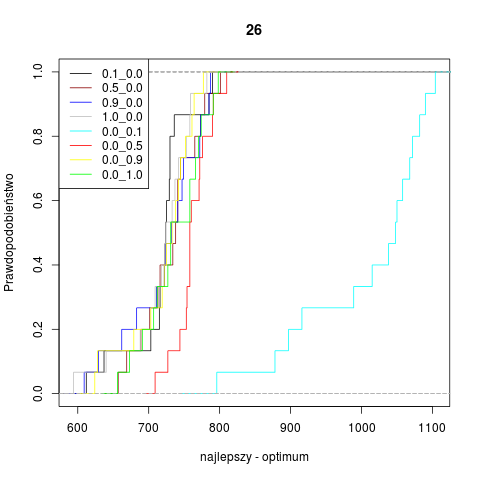
\includegraphics[width=.5\textwidth]{../tests/normal/26.png} }\quad
\subfigure[$p_m = 0$ - wyłączona mutacja]{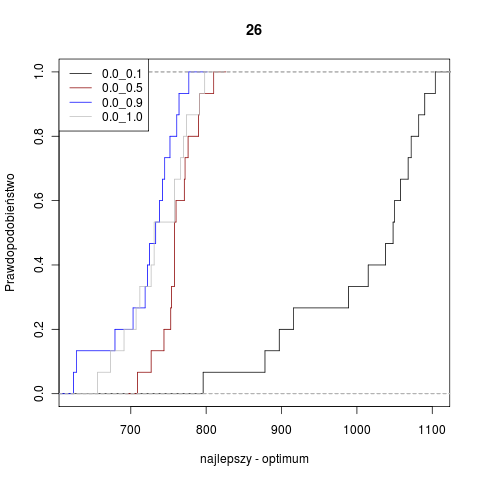
\includegraphics[width=.5\textwidth]{../tests/normal/26c.png} } 
}
\caption{Wpływ krzyżowania na działanie algorytmu - 26 miast}
\end{figure}

\begin{figure}[H]
\centering
\mbox{\subfigure[$p_m = 0,1$]{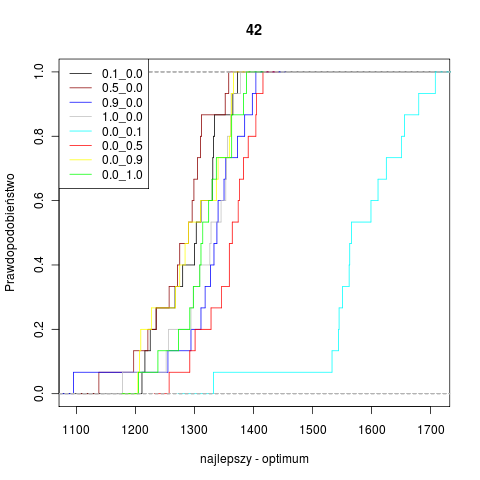
\includegraphics[width=.5\textwidth]{../tests/normal/42.png} }\quad
\subfigure[$p_m = 0$ - wyłączona mutacja]{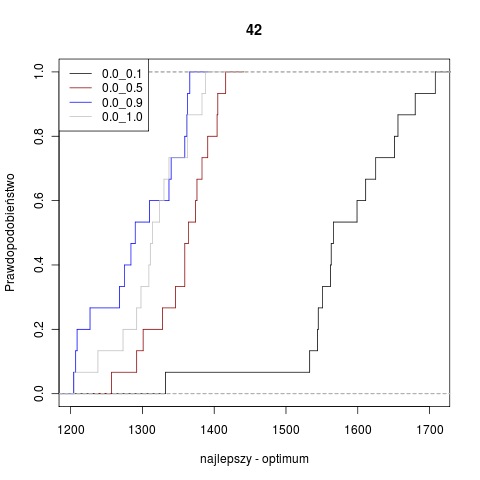
\includegraphics[width=.5\textwidth]{../tests/normal/42c.png} } 
}
\caption{Wpływ krzyżowania na działanie algorytmu - 42 miasta}
\end{figure}

\begin{figure}[H]
\centering
\mbox{\subfigure[$p_m = 0,1$]{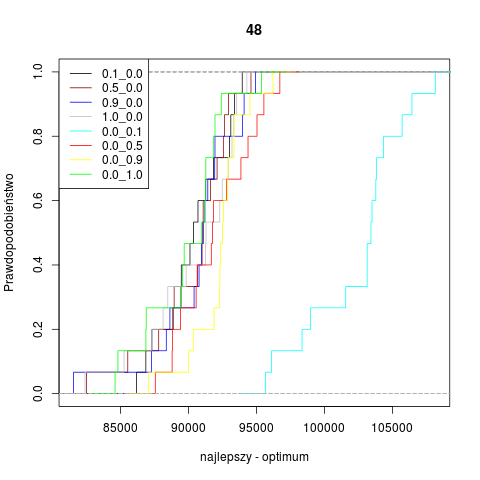
\includegraphics[width=.5\textwidth]{../tests/normal/48.png} }\quad
\subfigure[$p_m = 0$ - wyłączona mutacja]{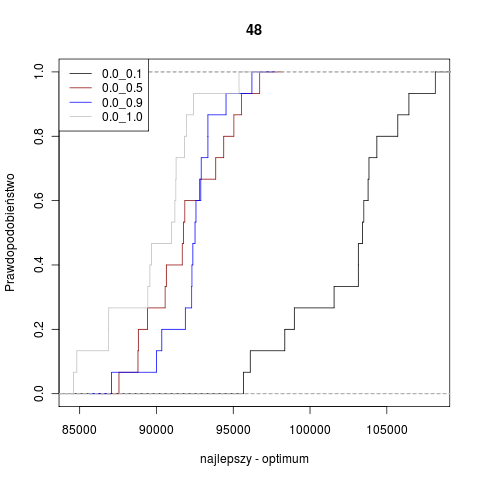
\includegraphics[width=.5\textwidth]{../tests/normal/48c.png} } 
}
\caption{Wpływ krzyżowania na działanie algorytmu - 48 miast}
\end{figure}

\subsection{Porównanie z algorytmem zachłannym}
	\subsubsection{Algorytm zachłanny}
	\subsubsection{Populacja algorytmu ewolucyjnego inicjowana wynikiem działania algorytmu zachłannego}
\begin{figure}[H]
\centering
\mbox{\subfigure[17 miast]{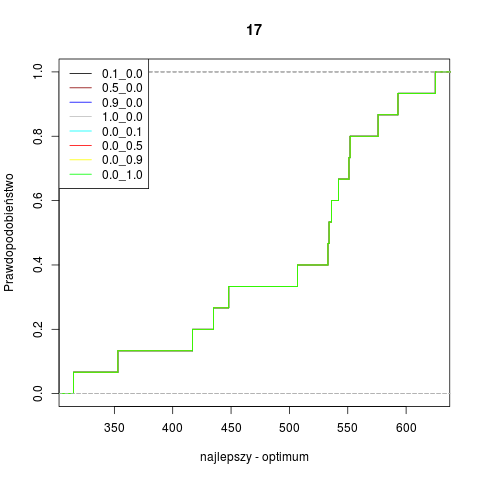
\includegraphics[width=.5\textwidth]{../tests/greedy_init/17.png} }\quad
\subfigure[26 miast]{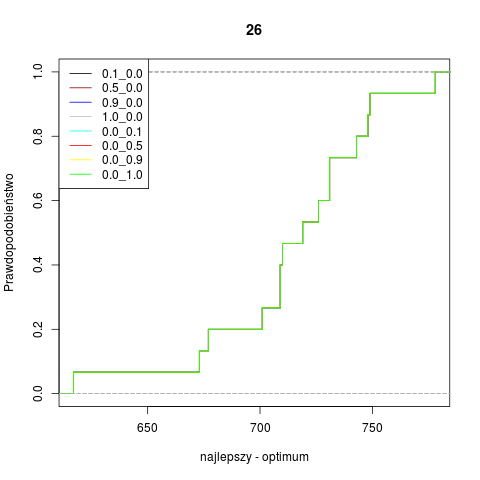
\includegraphics[width=.5\textwidth]{../tests/greedy_init/26.png} } 
}
\mbox{\subfigure[42 miasta]{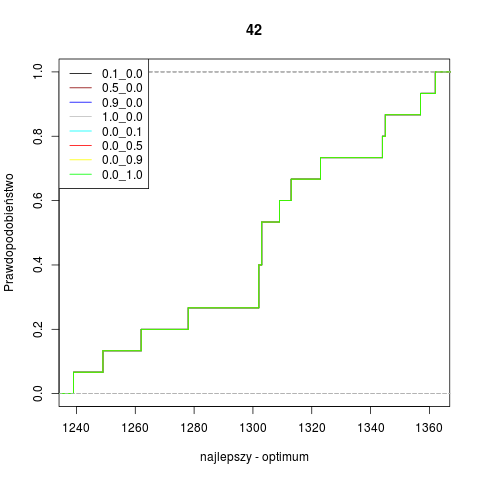
\includegraphics[width=.5\textwidth]{../tests/greedy_init/42.png} } 
\subfigure[48 miast]{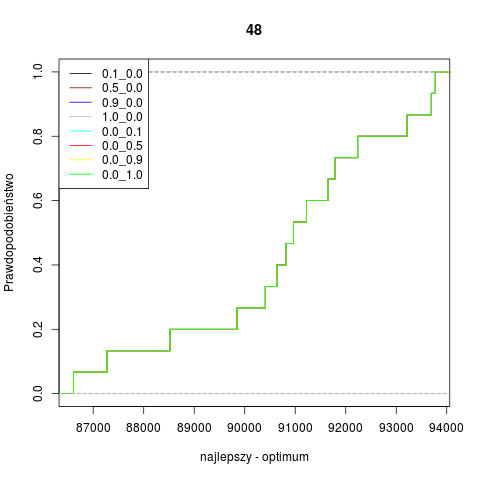
\includegraphics[width=.5\textwidth]{../tests/greedy_init/48.png} } 
}
\caption{Populacja algorytmu ewolucyjnego inicjowana wynikiem działania algorytmu zachłannego}
\end{figure}
\section{Wnioski}
 
\nocite{*}
\bibliographystyle{plain}
\bibliography{references}
\end{document}
